\documentclass{beamer}

%\usetheme{AnnArbor}
\usetheme{Boadilla}
\usecolortheme{whale}

\usepackage[utf8]{inputenc}
\graphicspath{{../Graphics/}}

\usepackage[absolute,overlay]{textpos}
\setlength{\TPHorizModule}{1pt}
\setlength{\TPVertModule}{1pt}
\usepackage{calc}

%Information to be included in the title page:
\title{Heat Energy Sources in Canada}
\author[Team 9]{Team 9: Noah Bolohan, Anton Iatcenko, Ryan Thiessen, Yakine Bahri, Benjamin MacAdam, Alireza Yazdani}
\institute[]{Math\textsuperscript{Industry}}

\date{August 2020}

\titlegraphic{
\includegraphics[width=2cm]{pims_logo.png}}



\begin{document}

\frame{\titlepage}


\begin{frame}
\frametitle{Team Members}

\begin{minipage}[b]{0.3\textwidth}

\end{minipage}
\begin{minipage}[b]{0.7\textwidth}

\end{minipage}

\end{frame}


\begin{frame}
\frametitle{Team Members}


\end{frame}





\begin{frame}
\frametitle{The Data Set (Yakine)}
\textbf{Primary heating systems and types of energy sources} : A table contains 2304 series, with data for the years 2013, 2015 and 2017
It contains data described by the following dimensions:
\begin{itemize}
\item Geography (48 items: Canada; Newfoundland and Labrador; Prince Edward Island; Nova Scotia; ...)
\item Primary heating system and type of energy (48 items: All primary heating systems; Electricity; Natural gas; Oil; ...).
\end{itemize}
\textbf{Source} : https://open.canada.ca/data/en/dataset/ec3282b6-013f-41b1-aa63-24ad8bda79ee
\end{frame}


\begin{frame}
\frametitle{Primary heating types in Canada: 2013-2017}
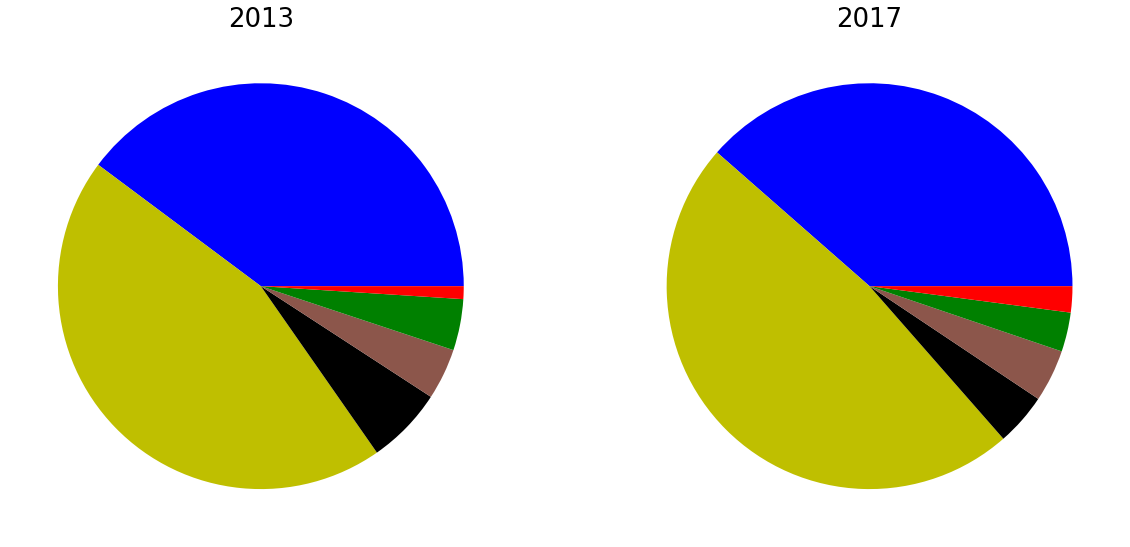
\includegraphics[width=\textwidth]{Canada20132017.png}\\
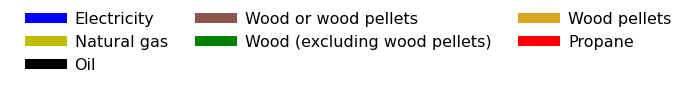
\includegraphics[width=\linewidth]{leg_bar.png}
\end{frame}



\begin{frame}
\frametitle{Change Over Time I (Anton)}
\begin{center}
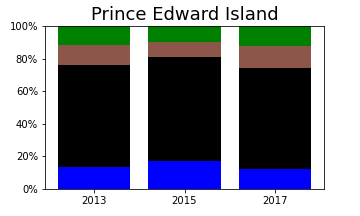
\includegraphics[width=0.5\linewidth]{pe.png}%
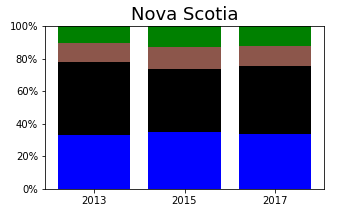
\includegraphics[width=0.5\linewidth]{ns.png}\\
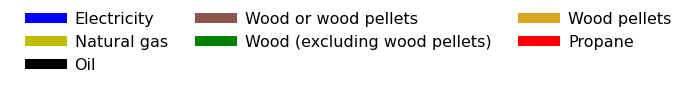
\includegraphics[width=0.9\linewidth]{leg_bar.png}
\end{center}
\end{frame}


\begin{frame}
\frametitle{Change Over Time II (Anton)}
\vspace{-10pt}
\begin{center}
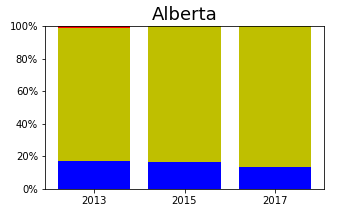
\includegraphics[width=0.48\linewidth]{ab.png}%
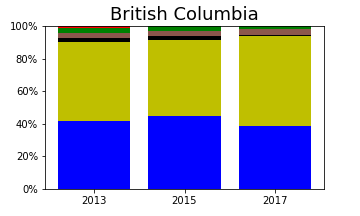
\includegraphics[width=0.48\linewidth]{bc.png}\\
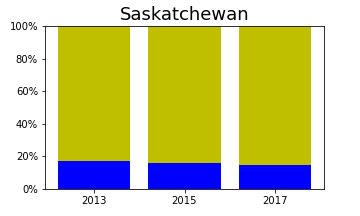
\includegraphics[width=0.48\linewidth]{sk.png}%
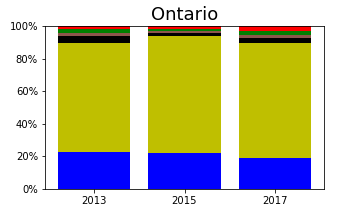
\includegraphics[width=0.48\linewidth]{on.png}\\
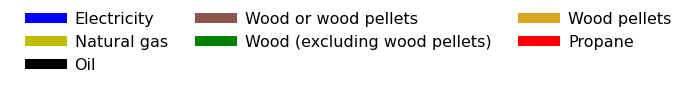
\includegraphics[width=0.9\linewidth]{leg_bar.png}
\end{center}
\end{frame}


\begin{frame}
\frametitle{Change Over Time III (Anton)}
\vspace{-10pt}
\begin{center}
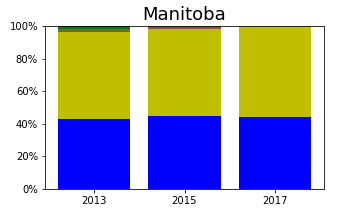
\includegraphics[width=0.48\linewidth]{mn.png}%
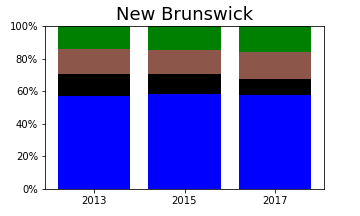
\includegraphics[width=0.48\linewidth]{nb.png}\\
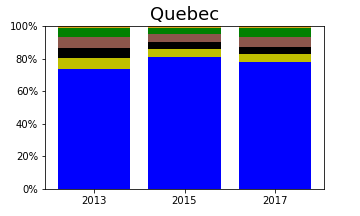
\includegraphics[width=0.48\linewidth]{qc.png}%
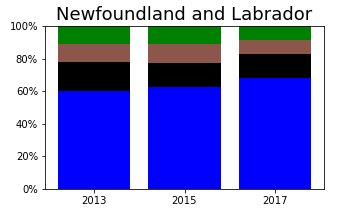
\includegraphics[width=0.48\linewidth]{nl.png}\\
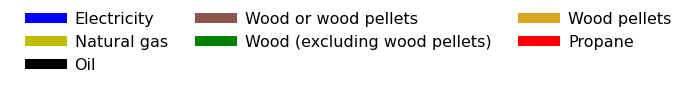
\includegraphics[width=0.9\linewidth]{leg_bar.png}
\end{center}
\end{frame}



\begin{frame}
\frametitle{Province Groupings (Anton)}


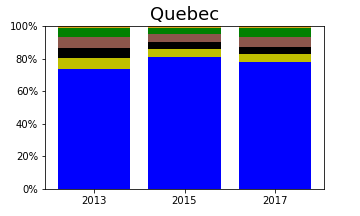
\includegraphics[width=0.33\linewidth]{qc.png}%
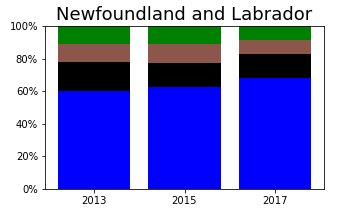
\includegraphics[width=0.33\linewidth]{nl.png}%
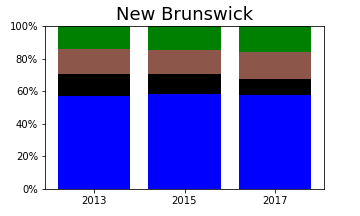
\includegraphics[width=0.33\linewidth]{nb.png}\\[10pt]
%
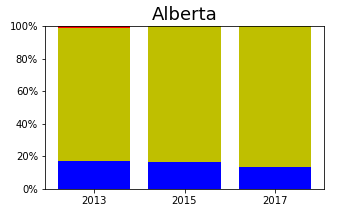
\includegraphics[width=0.33\linewidth]{ab.png}%
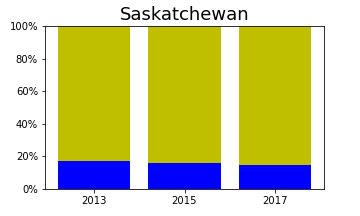
\includegraphics[width=0.33\linewidth]{sk.png}%
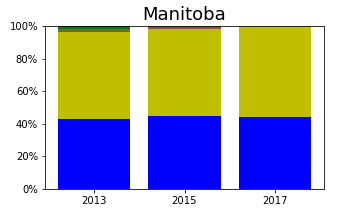
\includegraphics[width=0.33\linewidth]{mn.png}\\[10pt]
%
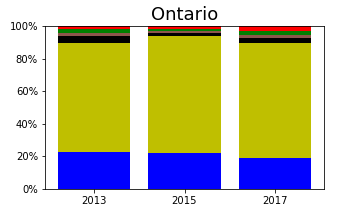
\includegraphics[width=0.25\linewidth]{on.png}%
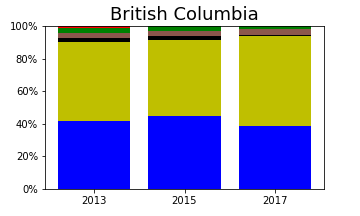
\includegraphics[width=0.25\linewidth]{bc.png}%
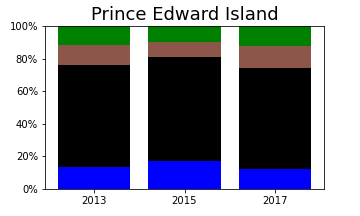
\includegraphics[width=0.25\linewidth]{pe.png}%
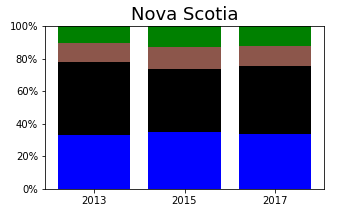
\includegraphics[width=0.25\linewidth]{ns.png}


\end{frame}


\begin{frame}

\frametitle{Cause of the Groupings: Natural Gas}

\begin{minipage}[b]{0.2\textwidth}
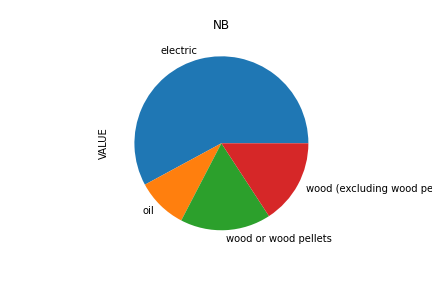
\includegraphics[width=0.8\textwidth, trim={120pt 50pt 110pt 40pt}, clip]{Ben_Images/NB.png}\\
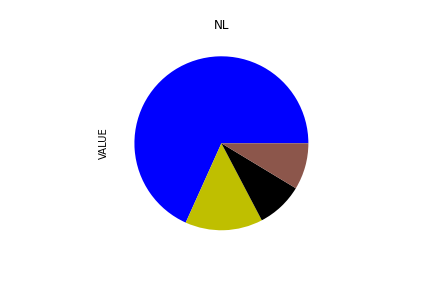
\includegraphics[width=0.8\textwidth, trim={120pt 50pt 110pt 40pt}, clip]{Ben_Images/NL.png}%
\end{minipage}%
%
%
\begin{minipage}[b]{0.55\textwidth}
\begin{center}
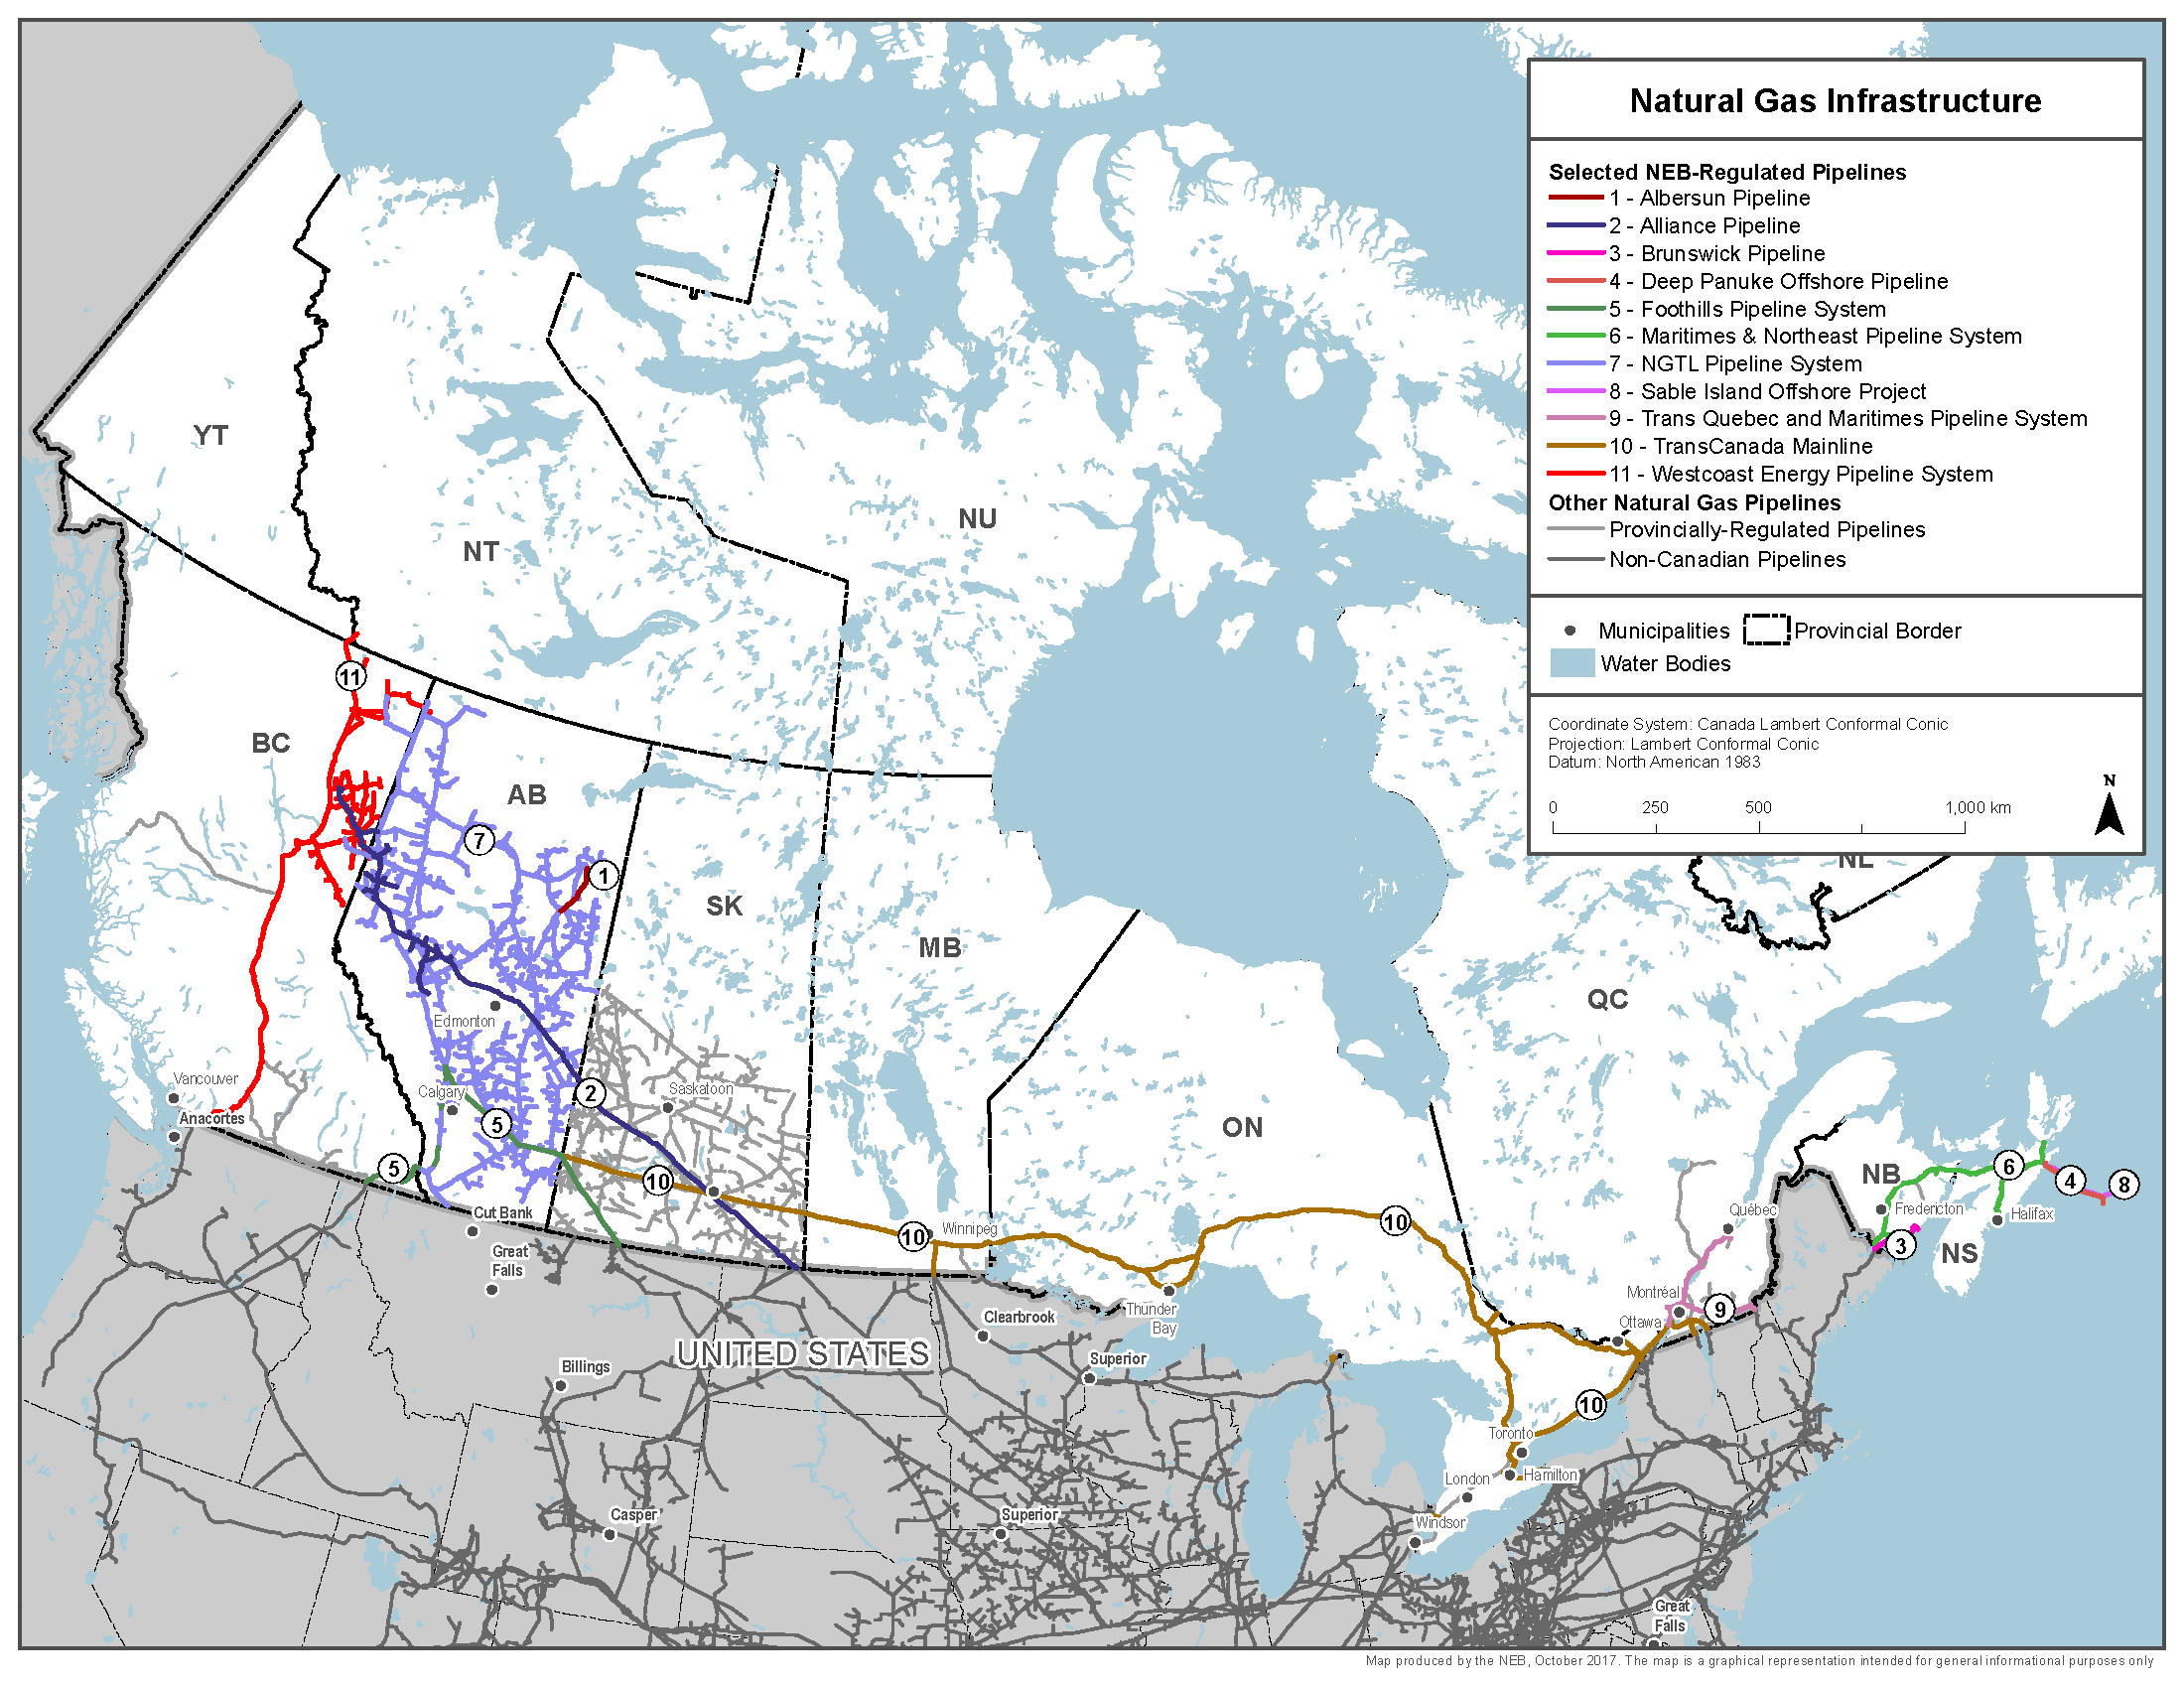
\includegraphics[width=\textwidth, trim={10 80pt 240pt 220pt}, clip]{natural_gas_pipeline_natural_resources_canada}
\end{center}
\end{minipage}



%\vspace{-10pt}

\small
\begin{itemize}
	\item SK, AB, and parts of BC have an extensive natural gas infrastructure.
	\item MB and ON have access to the natural gas TransCanada pipeline.
\end{itemize}
\normalsize
\end{frame}


\begin{frame}
\frametitle{Cause of the Groupings: Electricity (Alireza)}
\begin{center}
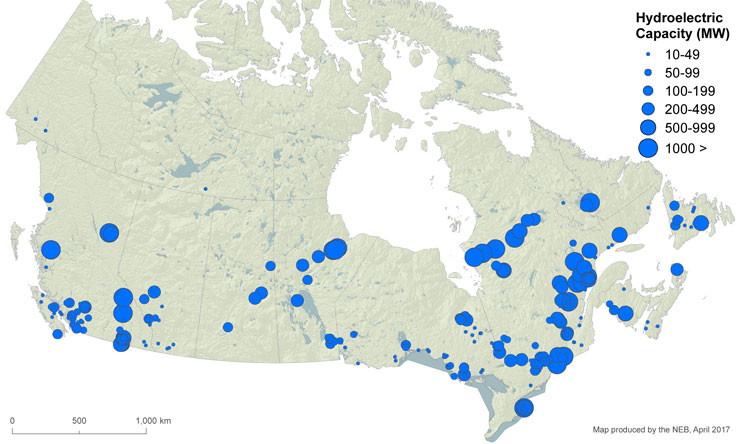
\includegraphics[width=0.6\textwidth]{hydroPower.jpg}
\small
\end{center}
\begin{itemize}
	\item QC: large hydroelectric capacity
	\item  NL and NB: close to QC, no access to natural gas  
\end{itemize}
\normalsize
\end{frame}











\begin{frame}
\frametitle{Cause of the Groupings: Atlantic Provinces (Ben)}

\begin{center}
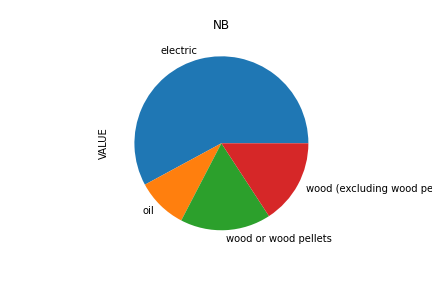
\includegraphics[width=0.25\linewidth, trim={120pt 50pt 110pt 10pt}, clip]{Ben_Images/NB.png}%
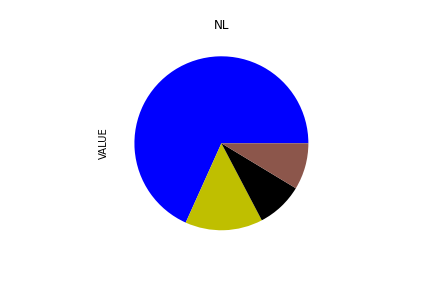
\includegraphics[width=0.25\linewidth, trim={120pt 50pt 110pt 10pt}, clip]{Ben_Images/NL.png}%
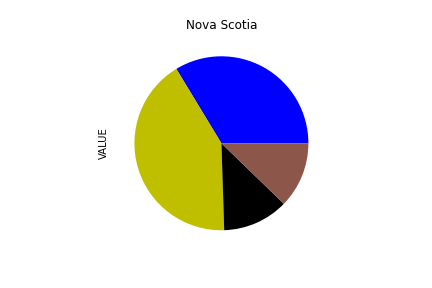
\includegraphics[width=0.25\linewidth, trim={120pt 50pt 110pt 10pt}, clip]{Ben_Images/NS.png}%
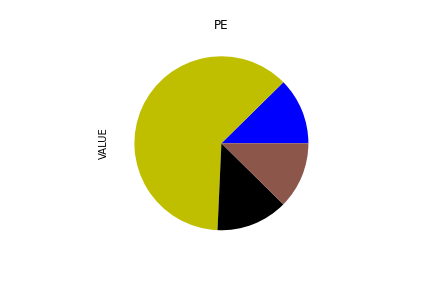
\includegraphics[width=0.25\linewidth, trim={120pt 50pt 110pt 10pt}, clip]{Ben_Images/PE.png}\\[10pt]
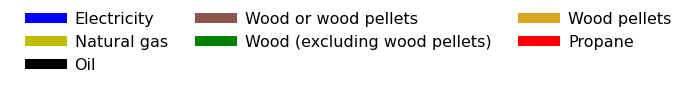
\includegraphics[width=0.8\linewidth]{leg_bar.png}
\end{center}

Same story in Atlantic region:
	\begin{itemize}
		\item Newfoundland, New Brunswick: access to hydro, use electric.
		\item Prince Edward Island, Nova Scotia: no hydro access, use oil.
	\end{itemize}

\end{frame}


















\begin{frame}
\frametitle{Summary}

No change over time.

The dependence is predominantly geographic.

Thanks for your attention.

\end{frame}













\end{document}
